\newpage
\begin{center}
    \Huge{\textbf{\underline{II.Exercise 3}}}
\end{center}

\vspace{0.45cm}

\begin{center}
    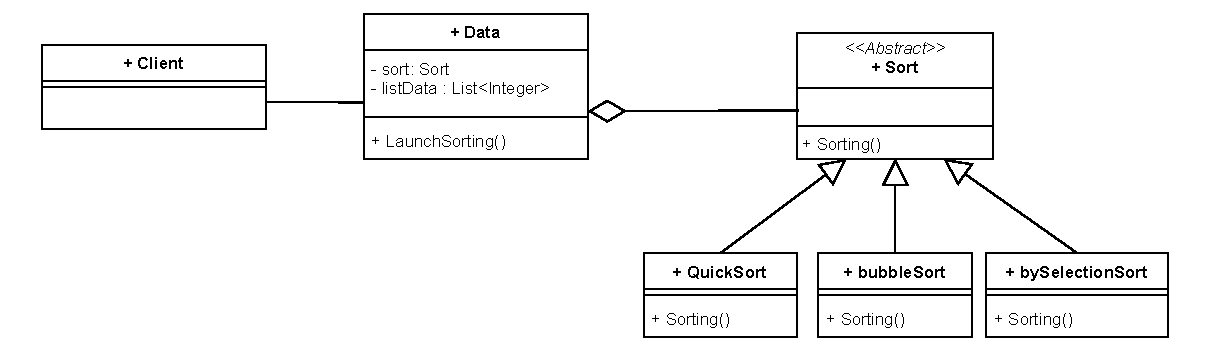
\includegraphics[height=0.18\textheight]{Exercices/2.EX3/ex3.drawio.pdf}
\end{center}

\vspace{0.25cm}

\begin{prettyBox}{Explication}{myblue}
The context here is the \texttt{Data} class, which holds the list of integers to be sorted. 
At runtime, the user can choose between different sorting methods interchangeably. 
Therefore, the \texttt{Sort} class is the abstract strategy, and the different sorting methods 
inherit from it.
\end{prettyBox}

